% % % % % % % % % % % % % % % % % % % % % % % % % % %
% IS&T Template 
% Patrick Vandewalle
% January 2006
% % % % % % % % % % % % % % % % % % % % % % % % % % %

%%%%%%%%%%%%%%%%%%%%%%%%%%%%%%%%%%
% Document class
%%%%%%%%%%%%%%%%%%%%%%%%%%%%%%%%%%
\documentclass[letterpaper,twocolumn,fleqn]{article} 

%%%%%%%%%%%%%%%%%%%%%%%%%%%%%%%%%%
% Packages
%%%%%%%%%%%%%%%%%%%%%%%%%%%%%%%%%%
\usepackage{ist}
% add other packages here
\usepackage{float} %forza
\usepackage{wrapfig} %forza
\usepackage{minted}

\pagestyle{empty}                % no page numbers is default

%%%%%%%%%%%%%%%%%%%%%%%%%%%%%%%%%%
% Title and Authors
%%%%%%%%%%%%%%%%%%%%%%%%%%%%%%%%%%

\title{ Designing a tone-shaping circuit for a guitar pedal }
\author{ Juan R. Ortiz; Pomona, California}
\date{\today} % date has an empty field.
% correct for bad hyphenation here
% \hyphenation{}

%%%%%%%%%%%%%%%%%%%%%%%%%%%%%%%%%%
% Begin document
%%%%%%%%%%%%%%%%%%%%%%%%%%%%%%%%%%
\begin{document} 
\maketitle 
\thispagestyle{empty} % prevents the first page to be numbered

%%%%%%%%%%%%%%%%%%%%%%%%%%%%%%%%%%
% Abstract
%%%%%%%%%%%%%%%%%%%%%%%%%%%%%%%%%%

\begin{abstract}
This article presents a practical application of Newton’s Method to design a tone‑shaping RC low‑pass filter used in guitar effects pedals. Beginning with a target cutoff frequency of 1kHz and a fixed 10k$\Omega$ resistor, the task is to determine the required capacitance by finding the root. The analysis involves typical audio‑circuit design, including an established standard 1nF–100nF capacitance range commonly used in analog signal paths. By defining the filter equation and its derivative, Newton’s Method will be implemented in Python to efficiently converge an acceptable solution. The resulting capacitor value of 16nF aligns with established tone‑shaping practices found in classic pedal circuitry such as the Big Muff, Tube Screamer, and Swollen Pickle.
\end{abstract}

\section{Objective}
\label{sec:intro}
The objective is to determine the capacitor value required to achieve a 1kHz cutoff frequency in a guitar‑pedal RC low‑pass filter. This work aims to demonstrate how numerical modeling techniques can be applied to practical analog‑audio design.

\section{Method}
In order to implement Newton's method, the functions must be defined given the parameters of a low-pass filter.
\vspace{0.1in}
\\The cutoff frequency of a simple RC low‑pass filter is:
\[\hspace{0.8in}
f_c = \frac{1}{2\pi RC}
\]
\vspace{0.05in}
This can be solved by rearranging the equation in root-finding form:
\[\hspace{0.8in}
g(C) = \frac{1}{2\pi RC} - f_c = 0
\]
\vspace{0.05in}
Next define the function and it's derivative:
\vspace{0.1in}
\[\hspace{0.8in}
f(C) = \frac{1}{2\pi RC} - f_c
\]
\[\hspace{0.8in}
f'(C) = -\frac{1}{2\pi RC^2}
\]
In the guitar pedal world and analog audio circuits, the capacitance
you choose in the signal path has a huge impact on the character of
the sound.

\vspace{0.05in}
The standard capacitance for tone-shaping can range from 1nF-
100nF, which will directly reflect electrical behavior and musical
intent
\vspace{0.1in}

\noindent Provided this standard range, a few assumptions can be made in order to solve the defined function.
%\vspace{-0.5in}
{\small
\begin{itemize}
    \item The plot interval: \{START, STOP\} = \{1nF, 100nF\} = \{1e-9, 1e-7\}
    \item Accuracy and tolerance: PRECISION = 1nF = 1e-9
    \item Initial guess: $x_0$ = 10nF = 1e-8
    \item Iterations: MAX\_STEPS = 20 (NM converges fast)
\end{itemize}}
%\vspace{-0.5in}
In Python the custom tool for solving by Newton's Method is scripted as:
%\vspace{-0.5in}
\begin{minted}[fontsize=\normalsize]{python}
def solve_newton_method(self, f, 
    df, x0, tolerance, max_steps
):
    x = x0

    for i in range(1, max_steps + 1):
        dfx = df(x)
        if dfx == 0:
            return x, i, -1

        fx = f(x)
        x_new = x - fx / dfx

        if abs(x_new - x) < tolerance:
            return x_new, i, 0

        x = x_new

    return x, max_steps, -2
\end{minted}
%\vspace{-0.5in}
With the method in place and the solver validated, I can now analyze the computed values.
\section{Result}
Figure \ref{fig:1} shows the low‑pass filter function over the 1nF–100nF range and the root found using Newton’s Method. The marked root 
gives the capacitance that meets the 1kHz cutoff and confirms a single valid solution within the design interval.
%\clearpage
\begin{figure}[H]
    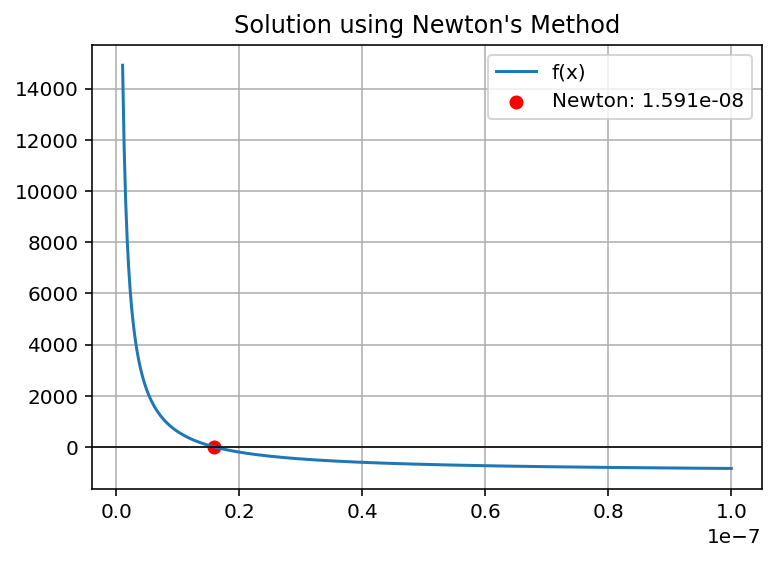
\includegraphics[width=1.0\linewidth]{NumMet_Newton_GTRPDL.png}
    \caption{Plot for solving the LPF capacitance through Python}
    \label{fig:1}
\end{figure}

The solution of approximately 16$nF$, is reasonably close to our initial 10$nF$ estimate. This mid‑range value is typical in tone‑shaping stages, providing the gentle high‑frequency roll‑off found in classic pedals such as the Big Muff, Tube Screamer, and Swollen Pickle. 
\vspace{0.15in}

\noindent Figure \ref{fig:2} shows the 1979 TS808 circuit designed by Susumu Tamura, which employs a similar low‑pass filtering approach to the one analyzed in this work

\begin{figure}[H]
    
\includegraphics[width=1.0\linewidth]{unit01/TS808.jpg}
    \caption{1979 TS808 Classic Overdrive Tubescreamer}
    \label{fig:2}
\end{figure}

%%%%%%%%%%%%%%%%%%%%%%%%%%%%%%%%%%%% 
\clearpage
% Overall Document Guidelines: Head
%%%%%%%%%%%%%%%%%%%%%%%%%%%%%%%%%%%%
\section{Overall Document Guidelines: Head}
\label{sec:intro}

Clear document of any fonts other than Times, Arial, and Symbol. The
paper should be formatted using the tags provided in the template,
i.e., title, author, section, subsection, subsubsection, eq./fig.,
references, etc.  in a 2 column format on US letter size paper ($8.5
\times 11$ inches, or $21.6 \times 27.9$ cm).

The left and right margins are set automatically to .75 inch (1.90 cm),
and the top and bottom margins to 1.0 inch (2.54 cm). The document is in
a 2-column format with column widths set at 3.38 inch (8.57 cm) and the
gutter -the space between columns- at .25 inch (0.635 cm).

Papers should be a maximum of 4-6 pages; longer papers will be
returned for revision. Please do not place folios or page numbers in
your paper. That information is inserted when we assemble the book.


%%%%%%%%%%%%%%%%%%%%%%%%%%%%%%%%%%
% Graphics and Equations
%%%%%%%%%%%%%%%%%%%%%%%%%%%%%%%%%%
\section{Graphics and Equations}
Graphics and equations should fit within one column (3.38 inches
wide), but full width (7 inch) figures are also acceptable. Equations,
figures and figure captions each have their own style tags. Equations
are numbered using parentheses flushed right as shown below.

\begin{equation}
\label{eq:ist}
\textrm{IS\&T} + \textrm{members} \times \textrm{Confs.} = \textrm{Success}
\end{equation}


\subsection{Helpful Hints and Style Tags: Subhead}
For a complete listing of the style tags for use in this template
refer to Table \ref{tab:fonts}. These are the style tags for
conference proceedings; if you use the wrong template/style tags your
paper will be sent back to you to be reformatted.  All of these forms
and templates related to the publication of conference papers are
available at

www.imaging.org/conferences/guidelines.cfm. 

Select the specific conference and download the Authors Kit. The
template may vary from one conference to another.

The template is set up for MS Word and LaTeX. Please check the paper
carefully to confirm that the styles have been applied correctly, then
print it out and double check to ensure that the paper appears as
intended.

\begin{table}[!h]
\caption{Style Tag Table: Table head}
\label{tab:fonts}
\begin{center}       
\begin{tabular}{|p{0.45\columnwidth}|p{0.45\columnwidth}|} 
\hline
1. Title& title environment \\ \hline
2. Byline: & \\
Author/Affiliation & author environment \\ \hline
3. Head & section environment \\ \hline
4. Subhead & subsection environment \\ \hline
5. Tertiary head & subsubsection environment \\ \hline
6. Abstract & abstract environment \\ \hline 
& \\ \hline
7. Body & regular text\\ \hline
8. Equation & equation environment\\ \hline
9.1 Figure & align left \\ \hline
9.2 Figure caption & caption environment \\ \hline
10.1 Table head & caption environment \\ \hline
10.2 Table text & tabular environment \\ \hline
11. References & bibliography + 
command \emph{small} to have a 1pt smaller font\\ \hline
12. Author Bio text & biography environment\\ \hline
13.1 List, bullet & itemize environment\\ \hline
13.2 List, numbered & enumerate environment \\ \hline
\end{tabular}
\end{center}
\end{table} 

%%%%%%%%%%%%%%%%%%%%%%%%%%%%%%%%%%
% Submitting Your Paper
%%%%%%%%%%%%%%%%%%%%%%%%%%%%%%%%%%

\section{Submitting Your Paper}
The submission of your paper has to be performed through the IS\&T
submission website. Authors receive a login for this site by e-mail.
Papers can be submitted in Postscript, Word, or WordPerfect format,
and will be converted to PDF by the submission server. Please
carefully review the generated PDF and verify that all the text,
equations, figures and tables are displayed correctly before approving
its submission.

\subsection{Margins in LaTeX}
Because of the differences between dvips conversion utilities, the
margins of your generated PDF document might vary. Please print
your document, and verify its margins. If they are incorrect, please
adapt the sizes of the margins in the file \emph{ist.sty}. Typically the
top margin should be decreased.

\begin{table}[!h]
\caption{Document Specs: Table head}
\label{tab:specs}
\begin{center}       
\begin{tabular}{p{0.35\columnwidth}p{0.55\columnwidth}} 
Paper Size & US Letter \\
Left/right margin & .75 inch (1.90 cm) \\
Top/bottom margin & 1 inch (2.54 cm) \\
Columns & 2 at 3.38 inch (8.57 cm) wide. \\
 & Spacing between columns: 0.25 inch (0.635 cm)
\end{tabular}
\end{center}
\end{table} 

\begin{figure}[!hb]
  
\includegraphics[width=0.3\columnwidth]{logo.png}
  \caption{IS\&T logo.}
  \label{Figure:logo}
\end{figure}

Please contact IS\&T with any questions or requests for assistance in
helping prepare the paper. We look forward to having your paper
presented at the conference and published in the conference
proceedings.

\begin{figure}[!hb]
  
\includegraphics[width=0.3\columnwidth]{logo.png}
  \caption{IS\&T logo.}
  \label{Figure:logo}
\end{figure}

%%%%%%%%%%%%%%%%%%%%%%%%%%%%%%%%%%
% Reference Preparation
%%%%%%%%%%%%%%%%%%%%%%%%%%%%%%%%%%

\section{Reference Preparation}
Use the standard LaTeX \emph{cite} command for references in the
text. You can then use the standard bibliography command to generate
the list of references. Add the command \emph{small} before the
bibliography to give it the right font size.  Reference \cite{bib1}
style should be used for books, Reference \cite{bib2} style should be
used for Journals, and Reference \cite{bib3} style should be used for
Proceedings.

%\section{Acknowledgments} 
%add the acknowledgement section here

% To start a new column (but not a new page) and help balance the last-page
% column length use \vfill\pagebreak.

%%%%%%%%%%%%%%%%%%%%%%%%%%%%%%%%%%
% Bibliography
%%%%%%%%%%%%%%%%%%%%%%%%%%%%%%%%%%

\small
\begin{thebibliography}{9}
\bibitem{bib1}John Doe, Recent Progress in Digital Halftoning II,
  IS\&T, Springfield, VA, 1999, pg. 173.
\bibitem{bib2}John Doe, Digital Imaging, J. Imaging. Sci. and
  Technol., 42, 112 (1998).
\bibitem{bib3}John Doe, An Inexpensive Micro-Goniophotometry You Can
  Build, Proc. PICS, pg. 179. (1998).
\end{thebibliography}

%%%%%%%%%%%%%%%%%%%%%%%%%%%%%%%%%%
% Biography
%%%%%%%%%%%%%%%%%%%%%%%%%%%%%%%%%%

\begin{biography}
Please submit a brief biographical sketch of no more than 75 words. 
Include relevant professional and educational information as shown 
in the example below.

Jane Doe received her BS in physics from the University of Nevada (1977) 
and her PhD in applied physics from Columbia University (1983). Since 
then she has worked in the Research and Technology Division at Xerox 
in Webster, NY. Her work has focused on the development of toner adhesion 
and transport issues. She is on the Board of  IS\&T and a member of APS 
and SPIE.
\end{biography}

\end{document} 
